%beamer

% Comment/uncomment this line to toggle handout mode
%\newcommand{\handout}{}

%% Beamer-Klasse im korrekten Modus
\ifdefined \handout
\documentclass[handout]{beamer} % Handout mode
\else
\documentclass{beamer}
\fi

%% UTF-8-Encoding
\usepackage[utf8]{inputenc}

\input{../framework/gbi-macros}
\usepackage[blue]{../framework/thwregex}
\usepackage{environ}
\usepackage{bm}
\usepackage{calc}
\usepackage{varwidth}
\usepackage{wasysym}
\usepackage{mathtools}


% Das ist der KIT-Stil
%\usepackage{../TutTexbib/beamerthemekit}
\usepackage[deutsch,titlepage0]{../framework/KIT/beamerthemeKITmod}
\TitleImage[width=\titleimagewd]{../figures/titlepage.jpg}
%\usetheme[deutsch,titlepage0]{KIT}

% Include PDFs
\usepackage{pdfpages}

% Libertine font (Original GBI font)
\usepackage{libertine}
%\renewcommand*\familydefault{\sfdefault}  %% Only if the base font of the document is to be sans serif

% Nicer math symbols
\usepackage{eulervm}
%\usepackage{mathpazo}
\renewcommand\ttdefault{cmtt} % Computer Modern typewriter font, see lecture slides.

\usepackage{csquotes}

%%%%%%

%% Schönere Schriften
\usepackage[TS1,T1]{fontenc}

%% Bibliothek für Graphiken
\usepackage{graphicx}

%% der wird sowieso in jeder Datei gesetzt
\graphicspath{{../figures/}}

%% Anzeigetiefe für Inhaltsverzeichnis: 1 Stufe
\setcounter{tocdepth}{1}

%% Hyperlinks
\usepackage{hyperref}
% I don't know why, but this works and only includes sections and NOT subsections in the pdf-bookmarks.
\hypersetup{bookmarksdepth=subsection} 

%\usepackage{lmodern}
\usepackage{colortbl}
\usepackage[absolute,overlay]{textpos}
\usepackage{listings}
\usepackage{forloop}
%\usepackage{algorithmic} % PseudoCode package 

\usepackage{tikz}
\usetikzlibrary{matrix}
\usetikzlibrary{arrows.meta}
\usetikzlibrary{automata}
\usetikzlibrary{tikzmark}
\usetikzlibrary{positioning}

% Why has no-one come up with this yet? I mean, seriously. -.-
\tikzstyle{loop below right} = [loop, out=-60,in=-30, looseness=7]
\tikzstyle{loop below left} = [loop, out=-150,in=-120, looseness=7]
\tikzstyle{loop above right} = [loop, out=60,in=30, looseness=7]
\tikzstyle{loop above left} = [loop, out=150,in=120, looseness=7]
\tikzstyle{loop right below} = [loop below right]
\tikzstyle{loop left below} = [loop below left]
\tikzstyle{loop right above} = [loop above right]
\tikzstyle{loop left above} = [loop above left]

% Needed for gbi-macros
\usepackage{xspace}

%%%%%%

%% Verbatim
\usepackage{moreverb}

%%%%%%%%%%%%%%%%%%%%%%%%%%%%%%%%%%%% Copy end

%% Tabellen
\usepackage{array}
\usepackage{multicol}
\usepackage{hhline}

%% Bibliotheken für viele mathematische Symbole
\usepackage{amsmath, amsfonts, amssymb}

%% Deutsche Silbentrennung und Beschriftungen
\usepackage[ngerman]{babel}

\usepackage{kbordermatrix}

% kbordermatrix settings
\renewcommand{\kbldelim}{(} % Left delimiter
\renewcommand{\kbrdelim}{)} % Right delimiter

\input{../config.tex}



% define custom \handout command flag if handout mode is toggled  #DirtyAsHellButWell...
\only<beamer:0>{\def\handout{}} %beamer:0 == handout mode

\newcommand{\R}{\mathbb{R}}
\newcommand{\N}{\mathbb{N}}
\newcommand{\Z}{\mathbb{Z}}
\newcommand{\Q}{\mathbb{Q}}
\newcommand{\BB}{\mathbb{B}}
\newcommand{\C}{\mathbb{C}}
\newcommand{\K}{\mathbb{K}}
\newcommand{\G}{\mathbb{G}}
\newcommand{\nullel}{\mathcal{O}}
\newcommand{\einsel}{\mathds{1}}
\newcommand{\Pot}{\mathcal{P}}
\renewcommand{\O}{\text{O}}

\def\word#1{\hbox{\textcolor{blue}{\texttt{#1}}}}
\let\literal\word
\def\mword#1{\hbox{\textcolor{blue}{$\mathtt{#1}$}}}  % math word
\def\sp{\scalebox{1}[.5]{\textvisiblespace}}
\def\wordsp{\word{\sp}}

%\newcommand{\literal}[1]{\textcolor{blue}{\texttt{#1}}}
\newcommand{\realTilde}{\textasciitilde \ }
\newcommand{\setsize}[1]{\ensuremath{\left\lvert #1 \right\rvert}}
\newcommand{\size}[1]{\setsize{#1}}  % Shame on you, TeXStudio...
\newcommand{\set}[1]{\left\{#1\right\}}
\newcommand{\tuple}[1]{\left(#1\right)}
\newcommand{\normalvar}[1]{\text{$#1$}}

% Modified by DJ
\let\oldemptyset\emptyset
\let\emptyset\varnothing % proper emptyset

\newcommand{\boder}{\ensuremath{\mathbin{\textcolor{blue}{\vee}}}\xspace}
\newcommand{\bund}{\ensuremath{\mathbin{\textcolor{blue}{\wedge}}}\xspace}
\newcommand{\bimp}{\ensuremath{\mathrel{\textcolor{blue}{\to}}}\xspace}
\newcommand{\bgdw}{\ensuremath{\mathrel{\textcolor{blue}{\leftrightarrow}}}\xspace}
\newcommand{\bnot}{\ensuremath{\textcolor{blue}{\neg}}\xspace}
\newcommand{\bone}{\ensuremath{\textcolor{blue}{1}}\text{}}
\newcommand{\bzero}{\ensuremath{\textcolor{blue}{0}}\text{}}
\newcommand{\bleftBr}{\ensuremath{\textcolor{blue}{\texttt{(}}}\text{}}
\newcommand{\brightBr}{\ensuremath{\textcolor{blue}{\texttt{)}}}\text{}}

% Fix of \b... commands:

\renewcommand{\boder}{\alor}
\renewcommand{\bund}{\aland}
\renewcommand{\bimp}{\alimpl}
\renewcommand{\bgdw}{\aleqv}
\renewcommand{\bnot}{\alnot}
\renewcommand{\bleftBr}{\alka}
\renewcommand{\brightBr}{\alkz}
\newcommand{\alA}{\word A}
\newcommand{\alB}{\word B}
\newcommand{\alC}{\word C}

\newcommand{\plB}{\plfoo{B}}
\newcommand{\plE}{\plfoo{E}}

\newcommand{\summe}[2]{\sum\limits_{#1}^{#2}}
\newcommand{\limes}[1]{\lim\limits_{#1}}

%\newcommand{\numpp}{\advance \value{weeknum} by -2 \theweeknum \advance \value{weeknum} by 2}
%\newcommand{\nump}{\advance \value{weeknum} by -1 \theweeknum \advance \value{weeknum} by 1}

\newcommand{\mycomment}[1]{}
\newcommand{\Comment}[1]{}

%% DISCLAIMER START 
% It is INSANELY IMPORTANT NOT TO DO THIS OUTSIDE BEAMER CLASS! IN ARTCILE DOCUMENTS, THIS IS VERY LIKELY TO BUG AROUND!
\makeatletter%
\@ifclassloaded{beamer}%
{
	% TODO 
	% no time... later.   (= never -.-)
	% redefine section to ignore multiple \section calls with the same title
}%
{
	\errmessage{ERROR: section command redefinition outside of beamer class document! Please contact the author of this code or read the F-ing disclaimer.}
}%
\makeatother%
%% DISCLAIMER END

\newcounter{abc}
\newenvironment{alist}{
  \begin{list}{(\alph{abc})}{
      \usecounter{abc}\setlength{\leftmargin}{8mm}\setlength{\labelsep}{2mm}
    }
}{\end{list}}


\newcommand{\stdarraystretch}{1.20}
\renewcommand{\arraystretch}{\stdarraystretch}  % for proper row spacing in tables

\newcommand{\morescalingdelimiters}{   % for proper \left( \right) typography
	\delimitershortfall=-1pt  
	\delimiterfactor=1
}

\newcommand{\centered}[1]{\vspace{-\baselineskip}\begin{center}#1\end{center}\vspace{-\baselineskip}}

% for \implitem and \item[bla] stuff to look right:
\setbeamercolor*{itemize item}{fg=black}
\setbeamercolor*{itemize subitem}{fg=black}
\setbeamercolor*{itemize subsubitem}{fg=black}

\setbeamercolor*{description item}{fg=black}
\setbeamercolor*{description subitem}{fg=black}
\setbeamercolor*{description subsubitem}{fg=black}

\renewcommand{\qedsymbol}{\textcolor{black}{\openbox}}

\renewcommand{\mod}{\mathop{\textbf{mod}}}
\renewcommand{\div}{\mathop{\textbf{div}}}

\newcommand{\ceil}[1]{\left\lceil#1\right\rceil}
\newcommand{\floor}[1]{\left\lfloor#1\right\rfloor}
\newcommand{\abs}[1]{\left\lvert #1 \right\rvert}
\newcommand{\Matrix}[1]{\begin{pmatrix} #1 \end{pmatrix}}
\newcommand{\braced}[1]{\left\lbrace #1 \right\rbrace}

% "something" placeholder. Useful for repairing spacing of operator sections, like `\sth = 42`.
\def\sth{\vphantom{.}}

\def\fract#1/#2 {\frac{#1}{#2}} % ! Trailing space is crucial!
\def\dfract#1/#2 {\dfrac{#1}{#2}} % ! Trailing space is crucial!

\newcommand{\Mid}{\;\middle|\;}

\let\after\circ



\def\·{\cdot}
\def\*{\cdot}
\def\?>{\ensuremath{\rightsquigarrow}}  % Fuck you, Latex
\def\~~>{\ensuremath{\rightsquigarrow}}  

\newcommand{\tight}[1]{{\renewcommand{\arraystretch}{0.76} #1}}
\newcommand{\stackedtight}[1]{\renewcommand{\arraystretch}{0.76} \begin{matrix} #1 \end{matrix} }
\newcommand{\stacked}[1]{\begin{matrix} #1 \end{matrix} }
\newcommand{\casesl}[1]{\delimitershortfall=0pt  \left\lbrace\hspace{-.3\baselineskip}\begin{array}{ll} #1 \end{array}\right.}
\newcommand{\casesr}[1]{\delimitershortfall=0pt  \left.\begin{array}{ll} #1 \end{array}\hspace{-.3\baselineskip}\right\rbrace}
\newcommand{\caseslr}[1]{\delimitershortfall=0pt  \left\lbrace\hspace{-.3\baselineskip}\begin{array}{ll} #1 \end{array}\hspace{-.3\baselineskip}\right\rbrace}

\def\q#1uad{\ifnum#1=0\relax\else\quad\q{\the\numexpr#1-1\relax}uad\fi}
% e.g. \q1uad = \quad, \q2uad = \qquad etc.

\newcommand{\qqquad}{\q3uad}
\newcommand{\minusquad}{\hspace{-1em}}

%% Placeholder utils
% \§{#1}   Saves #1 as placeholder and prints it
% \.       Prints an \hphantom with the size of the recalled placeholder.
\def\indentstring{}
\def\§#1{\def\indentstring{#1}#1}
\def\.{{$\hphantom{\text{\indentstring}}$}}
%% Placeholder utils end

\newcommand{\impl}{\ifmmode\ensuremath{\mskip\thinmuskip\Rightarrow\mskip\thinmuskip}\else$\Rightarrow$\fi\xspace}
\newcommand{\Impl}{\ifmmode\implies\else$\Longrightarrow$\fi\xspace}

\newcommand{\derives}{\Rightarrow}

\newcommand{\gdw}{\ifmmode\mskip\thickmuskip\Leftrightarrow\mskip\thickmuskip\else$\Leftrightarrow$\fi\xspace}
\newcommand{\Gdw}{\ifmmode\iff\else$\Longleftrightarrow$\fi\xspace}

% Legacy code from the algo tutorial slides. Perhaps useful. Try with care.
\mycomment{
	\newcommand{\impl}{\ifmmode\ensuremath{\mskip\thinmuskip\Rightarrow\mskip\thinmuskip}\else$\Rightarrow$\xspace\fi}  
	\newcommand{\Impl}{\ifmmode\implies\else$\Longrightarrow$\xspace\fi}
	
	\newcommand{\gdw}{\ifmmode\mskip\thickmuskip\Leftrightarrow\mskip\thickmuskip\else$\Leftrightarrow$\xspace\fi}
	\newcommand{\Gdw}{\ifmmode\iff\else$\Longleftrightarrow$\xspace\fi}
}
	
\newcommand{\gdwdef}{\ifmmode\mskip\thickmuskip:\Leftrightarrow\mskip\thickmuskip\else:$\Leftrightarrow$\xspace\fi}
\newcommand{\Gdwdef}{\ifmmode\mskip\thickmuskip:\Longleftrightarrow\mskip\thickmuskip\else:$\Longleftrightarrow$\xspace\fi}

\newcommand{\symbitemnegoffset}{\hspace{-.5\baselineskip}}
\newcommand{\implitem}{\item[\impl\symbitemnegoffset]}
\newcommand{\Implitem}{\item[\Impl\symbitemnegoffset]}


\newcommand{\forcenewline}{\mbox{}\\}

\newcommand{\bfalert}[1]{\textbf{\alert{#1}}}
\let\elem\in   % I'm a Haskell freak. Don't judge me. :P


\def\|#1|{\text{\normalfont #1}}  % | steht für senkrecht (anstatt kursiv wie sonst im math mode)


% proper math typography
\newcommand{\functionto}{\longrightarrow}
\renewcommand{\geq}{\geqslant}
\renewcommand{\leq}{\leqslant}
\let\oldsubset\subset
\renewcommand{\subset}{\subseteq} % for all idiots out there using subset

\newenvironment{threealign}{%
	\[
	\begin{array}{r@{\ }c@{\ }l}
}{%
	\end{array}	
	\]
}

\newcommand{\concludes}{ \\ \hline  }
\newcommand{\deduction}[1]{
	\begin{varwidth}{.8\linewidth}
		\begin{tabular}{>{$}c<{$}}
			#1
		\end{tabular}
	\end{varwidth}	
}

\definecolor{hoareorange}{rgb}{1,.85,.6}
\newcommand{\hoareassert}[1]{\setlength{\fboxsep}{1pt}\setlength{\fboxrule}{-1.4pt}\fcolorbox{white}{hoareorange}{\ensuremath{\{\;#1\;\}}}\setlength\fboxrule{\defaultfboxrule}\setlength{\fboxsep}{3pt}}

\newcommand{\mailto}[1]{\href{mailto:#1}{{\textcolor{blue}{\underline{#1}}}}}
\newcommand{\urlnamed}[2]{\href{#2}{\textcolor{blue}{\underline{#1}}}}
\renewcommand{\url}[1]{\urlnamed{#1}{#1}}

\newcommand{\hanging}{\hangindent=0.7cm}
\newcommand{\indented}{\hanging}


% \hstretchto prints #2 left-aligned into a box of the width of #1
\def\hstretchto#1#2{%
	\mbox{}\vphantom{#2}\rlap{#2}\hphantom{#1}%
}

\def\vstretchto#1#2{%
	\mbox{}\hphantom{#2}\smash{#2}\vphantom{#1}%
}

% \hstretchtocentered prints #2 centered into a box of the width of #1
\def\hstretchtocentered#1#2{%
	\mbox{}\vphantom{#2}\scalebox{0.5}{\hphantom{#1}}\clap{#2}\scalebox{0.5}{\hphantom{#1}}%
}

% vertical centering
\newcommand{\vertcenter}[1]{%
	\ensuremath{\vcenter{\hbox{#1}}}%
}


%requires \thisyear to be defined (s. config.tex)!
\edef\nextyear{\the\numexpr\thisyear+1\relax}


% --- \frameheight constant ---
\newlength\fullframeheight
\newlength\framewithtitleheight
\setlength\fullframeheight{.92\textheight}
\setlength\framewithtitleheight{.86\textheight}

\newlength\frameheight
\setlength\frameheight{\fullframeheight}

\let\frametitleentry\relax
\let\oldframetitle\frametitle
\def\newframetitle#1{\global\def\frametitleentry{#1}\if\relax\frametitleentry\relax\else\setlength\frameheight{\framewithtitleheight}\fi\oldframetitle{#1}}
\let\frametitle\newframetitle

\def\newframetitleoff{\let\frametitle\oldframetitle}
\def\newframetitleon{\let\frametitle\newframetitle}
% --- \frameheight constant end ---

\newcommand{\fakeframetitle}[1]{%
	\vspace{-2.05\baselineskip}%
	{\Large \textbf{#1}} \\%
	\smallskip
}



\newenvironment{headframe}{\Huge THIS IS AN ERROR. PLEASE CONTACT THE ADMIN OF THIS TEX CODE. (headframe env def failed)}{}
\RenewEnviron{headframe}[1][]{
	\begin{frame}\frametitle{\ }
		\centering
		\Huge\textbf{\textsc{\BODY} \\
		}
		\Large {#1}
		\frametitle{\ }
	\end{frame}
}


\makeatletter
% Provides color if undefined.
\newcommand{\colorprovide}[2]{%
	\@ifundefinedcolor{#1}{\colorlet{#1}{#2}}{}}
\makeatother


\colorprovide{lightred}{red!30}
\colorprovide{lightgreen}{green!40}
\colorprovide{lightyellow}{yellow!50}
\colorprovide{lightblue}{blue!10}
\colorprovide{beamerlightred}{lightred}
\colorprovide{beamerlightgreen}{lightgreen}
\colorprovide{beamerlightyellow}{lightyellow}
\colorprovide{beamerlightblue}{lightblue}
\colorprovide{fullred}{red!60}
\colorprovide{fullgreen}{green}
\definecolor{darkred}{RGB}{115,48,38}
\definecolor{darkgreen}{RGB}{48,115,38}
\definecolor{darkyellow}{RGB}{100,100,0}

\only<handout:0>{\colorlet{adaptinglightred}{beamerlightred}}
\only<handout:0>{\colorlet{adaptinglightgreen}{beamerlightgreen}}
\only<handout:0>{\colorlet{adaptinglightyellow}{beamerlightyellow}}
\only<handout:0>{\colorlet{adaptinglightblue}{beamerlightblue}}
\only<beamer:0>{\colorlet{adaptinglightred}{lightred}}
\only<beamer:0>{\colorlet{adaptinglightgreen}{lightgreen}}
\only<beamer:0>{\colorlet{adaptinglightyellow}{lightyellow}}
\only<beamer:0>{\colorlet{adaptinglightblue}{lightblue}}
\only<handout:0>{\colorlet{adaptingred}{lightred}}
\only<beamer:0>{\colorlet{adaptingred}{fullred}}
\only<handout:0>{\colorlet{adaptinggreen}{lightgreen}}
\only<beamer:0>{\colorlet{adaptinggreen}{fullgreen}}



\newcommand{\TrueQuestion}[1]{
	\TrueQuestionE{#1}{}
}

\newcommand{\YesQuestion}[1]{
	\YesQuestionE{#1}{}
}

\newcommand{\FalseQuestion}[1]{
	\FalseQuestionE{#1}{}
}

\newcommand{\NoQuestion}[1]{
	\NoQuestionE{#1}{}
}

\newcommand{\DependsQuestion}[1]{
	\DependsQuestionE{#1}{}
}

\newcommand{\QuestionVspace}{\vspace{4pt}}
\newcommand{\QuestionParbox}[1]{\begin{varwidth}{.85\linewidth}#1\end{varwidth}}
\newcommand{\ExplanationParbox}[1]{\begin{varwidth}{.97\linewidth}#1\end{varwidth}}
\colorlet{questionlightgray}{gray!23}
\let\defaultfboxrule\fboxrule

% #1: bg color
% #2: fg color short answer
% #3: short answer text
% #4: question
% #5: explanation
\newcommand{\GenericQuestion}[5]{
	\setlength\fboxrule{2pt}
	\only<+|handout:0>{\hspace{-2pt}\fcolorbox{white}{questionlightgray}{\QuestionParbox{#4} \quad\textbf{?}}}
	\visible<+->{\hspace{-2pt}\fcolorbox{white}{#1}{\QuestionParbox{#4} \quad\textbf{\textcolor{#2}{#3}}} \if\relax#5\relax\else\ExplanationParbox{#5}\fi} \\
	\setlength\fboxrule{\defaultfboxrule}
}

% #1: Q text
% #2: Explanation
\newcommand{\TrueQuestionE}[2]{
	\GenericQuestion{adaptinglightgreen}{darkgreen}{Wahr.}{#1}{#2}
}

% #1: Q text
% #2: Explanation
\newcommand{\YesQuestionE}[2]{
	\GenericQuestion{adaptinglightgreen}{darkgreen}{Ja.}{#1}{#2}
}

% #1: Q text
% #2: Explanation
\newcommand{\FalseQuestionE}[2]{
	\GenericQuestion{adaptinglightred}{darkred}{Falsch.}{#1}{#2}
}

% #1: Q text
% #2: Explanation
\newcommand{\NoQuestionE}[2]{
	\GenericQuestion{adaptinglightred}{darkred}{Nein.}{#1}{#2}
}

% #1: Q text
% #2: Explanation
\newcommand{\DependsQuestionE}[2]{
	\GenericQuestion{adaptinglightyellow}{darkyellow}{Je nachdem!}{#1}{#2}
}

% #1: Q text
% #2: Answer
\newcommand{\ContentQuestion}[2]{
	\GenericQuestion{adaptinglightblue}{black}{\minusquad}{#1}{#2}
}

\ifnum\thisyear=2021 \else \errmessage{Old ILIAS link inside preamble. Please update.} \fi

\newcommand{\ILIAS}{\urlnamed{ILIAS}{\myILIASurl}\xspace}
\newcommand{\Klausurtermin}{\myKlausurtermin\xspace}

\newcommand{\Socrative}{\ifdefined\mysocrativeroom \only<handout:0>{socrative.com $\quad \~~> \quad $ Student login \\ Raumname:  \mysocrativeroom\\ \medskip}\else\fi}

\newcommand{\thasse}[1]{
	\ifdefined\ThassesTut #1\xspace \else\fi
}
\newcommand{\daniel}[1]{
	\ifdefined\DanielsTut #1\xspace \else\fi
}
\newcommand{\thassedaniel}[2]{\ifdefined\ThassesTut #1\else\ifdefined\DanielsTut #2\fi\fi\xspace}

\ifdefined\ThassesTut \ifdefined\DanielsTut \errmessage{ERROR: Both ThassesTut and DanielsTut flags are set. This is most likely an error. Please check your config.tex file.} \else \fi \else \ifdefined\DanielsTut \else \errmessage{ERROR: Neither ThassesTut  nor DanielsTut flags are set. This is most likely an error. Please check your config.tex file.} \fi\fi

%\newcommand{\sgn}{\text{sgn}}

%%%%%%%%%%%% INHALT %%%%%%%%%%%%%%%%

%% Wochennummer
\newcounter{weeknum}

%% Titelinformationen
\title[GBI-Tutorium \mytutnumber, Woche \theweeknum]{Grundbegriffe der Informatik \\ Tutorium \mytutnumber}

\subtitle{Woche \theweeknum\xspace |\xspace\mydate{\theweeknum} \\ \myname \ \  \normalfont (\mailto{\mymail})}
\author[\myname]{\myname}
\institute{KIT -- Karlsruher Institut für Technologie}
\date{\mydate{\theweeknum}\ }

% Modified, DJ (better safe than sorry)
\AuthorTitleSep{ – }

%% Titel einfügen
\newcommand{\titleframe}{\frame{\titlepage}}

%% Alles starten mit \starttut{X}
\newcommand{\starttut}[1]{\setcounter{weeknum}{#1}\pdfinfo{
		/Author (\myname)
		/Title  (GBI-Tutorium \mytutnumber, Woche \theweeknum)
	}\titleframe\frame{\frametitle{Inhalt}\tableofcontents} \AtBeginSection[]{%
		\begin{frame}{Wo sind wir gerade?}
		\tableofcontents[currentsection]
	\end{frame}\addtocounter{framenumber}{-1}}}


\newcommand{\framePrevEpisode}{
\begin{headframe}
	\mylasttimestext
\end{headframe}
}

\newcommand{\lastframetitled}[6]{
	\frame{\frametitle{#6}
		\vspace{-#2\baselineskip}
		\begin{figure}[H]
			\centering
			\LARGE \textbf{\textsc{#5}} \\
			\vspace{.2\baselineskip}
			\includegraphics[#1]{#3}
			\vspace{-6pt}
			\begin{center}
				\small \url{#4} 
			\end{center}
		\end{figure} 
	}
}

% #1 number
% #2 title 
% #3 vspace (positive) without unit (\baselineskip)
\newcommand{\xkcdframe}[3]{
	\lastframetitled{width=.96\textwidth}{#3}{xkcd/#1}{http://xkcd.com/#1}{}{#2}
}

\newcommand{\xkcdframevert}[3]
{
	\lastframetitled{height=.96\frameheight}{#3}{xkcd/#1}{http://xkcd.com/#1}{}{#2}
}

% #1 number
% #2 title 
% #3 vspace (positive) without unit (\baselineskip)
% #4 \includegraphics[] optional parameters
\newcommand{\xkcdframecustom}[4]
{
	\lastframetitled{#4}{#3}{xkcd/#1}{http://xkcd.com/#1}{}{#2}
}

\newcommand{\slideThanks}{
	\begin{frame}
	\frametitle{Credits}
	\begin{block}{}
		An der Erstellung des Foliensatzes haben mitgewirkt:\\[1em]
		Daniel Jungkind \\
		Thassilo Helmold \\
		Philipp Basler \\
		Nils Braun \\
		Dominik Doerner \\
		Ou Yue \\
		Max Schweikart
	\end{block}
\end{frame}
}

%% Wörter DEPRECATED! DO NOT USE
\newcommand{\code}[1]{$\mathbf{#1}$}

\morescalingdelimiters

\begin{document}
\starttut{4}

\section{Organisatorisches}

\begin{frame}{Zu Übungsblatt \#2}
	Schnitt: \quad 9,9 / 19~P

	\begin{itemize}[<+->]
		\item 19 von 23 Tutanden haben etwas abgegeben. Weiter so!
		\item Die Korrektur und die Musterlösung findet ihr im ILIAS-Aufgaben-Objekt
		\item Nur die Person, die das Übungsblatt abgegeben hat, bekommt die Rückmeldung \impl tauscht euch aus!
		\item Ihr habt alle pünktlich abgegeben :)
		\item Notation lief um einiges besser, aber immer noch nicht perfekt
	\end{itemize}
\end{frame}

\begin{frame}{Zu Übungsblatt \#2}
	Die häufigsten Fehler:
	\begin{itemize}[<+->]
		\item Definiert alle Variablen, die ihr benutzt! \\
			z.B. wenn ihr schreiben wollt: \textit{aus $w(i)=0$ folgt $w(i) \not = 1$}, dann müsst ihr vorher irgendwo $w$ und $i$ definiert haben.
		\item Eine \textbf{Annahme} beschreibt etwas, das \textit{eigentlich} nicht unbedingt gelten muss, bei dem ihr aber \textit{annehmt}, dass es gilt.
		\implitem Benutzen bei Widerspruchsbeweisen und Fallunterscheidungen (\textit{Fall 1: $x=0$: ..., Fall 2: $x \not = 0$: ...})
		\implitem Nicht als Überschrift für Definitionen, Voraussetzungen und Beweise benutzen!
		\item Einfach Pfeile ($\leftarrow, \rightarrow, \leftrightarrow$) benutzt man nur bei der \textit{formalen} Betrachtung von Aussagenlogik!
		\implitem Für Folgerungen und Äquivalenzen im Beweis benutzt man Doppelpfeile ($\Rightarrow, \Leftarrow, \Leftrightarrow$).
		\item Behauptungen müsst ihr als solche kennzeichnen
	\end{itemize}
\end{frame}

\begin{frame}{Zu Übungsblatt \#2}
	Die häufigsten Fehler:
	\begin{itemize}[<+->]
		\item Kommutativität und Assoziativität zeigen
		\item Kommutativität und Assoziativität widerlegen
		\item Wir machen das jetzt nochmal zusammen
	\end{itemize}
\end{frame}

\framePrevEpisode

\begin{frame}{Kahoot!}
	\begin{itemize}[<+->]
		\item Kahoot! ist ein anonymes Online-Quiz
		\item Ihr bekommt Punkte für schnelles und richtiges raten
		\item Ich schalte das Quiz frei und ihr könnt über \url{https://kahoot.it} beitreten
		\item Das Kahoot! könnt ihr euch später nochmal unter diesem Link angucken: \\
			\url{https://create.kahoot.it/share/gbi-woche-3-einstieg/c0638af4-aaa2-4892-8916-a2eab442312d}
	\end{itemize}
\end{frame}

%\begin{frame}{Rückblick}
%	\begin{itemize}
%		\item \textbf{Aussagen} sind Sätze, die wahr oder falsch sind
%		\item Wir können Aussagen mit \textbf{Konnektiven} zusammenbauen: \\
%		$\bund, \boder, \bnot, \bimp$
%		\item \textbf{Aussagevariablen} helfen dabei, konkrete Inhalte zu ignorieren 
%		\item \textbf{Interpretationen} liefern Wahrheitswerte zu Variablen
%		\item $val_I(\*)$ liefert Wahrheitswert für ganze Formel (rekursiv)
%	\end{itemize}
%\end{frame}

%\begin{frame}[t]{Wahr oder Falsch?}
 %	% Socrative: https://b.socrative.com/teacher/#import-quiz/31489145
 %	\Socrative
 %	
 %	\TrueQuestion{Dieser Satz ist eine Aussage.}
 %	\FalseQuestionE{$\alA \boder \alB = \alB \boder \alA$}{Das sind syntaktisch verschiedene AL-Formeln!}
 %	\TrueQuestion{$\alA \boder \alB \equiv \alB \boder \alA$}
 %	% \TrueQuestion{Der AL-Kalkül ist vollständig und korrekt.}  % Wurde noch gar nicht erklärt...!?
 %	\TrueQuestion{Es gibt unendlich viele Axiome im Aussagenkalkül.}
 %	\FalseQuestion{$\bleftBr \word G \bimp \word H \brightBr \; \vdash \;  \bleftBr \word H \bimp \word G \brightBr$}
 %	\FalseQuestion{Induktion kann man nur auf Zahlen anwenden.}
%\end{frame}


\section{Aussagenlogik}

%\thasse{ % No time this year...
%	\frame{
%		\frametitle{Ein bekanntes Logikrätsel}
%		\vspace{-2pt}
%		\begin{figure}[H]
%			\centering
%			\only<1|handout:1>{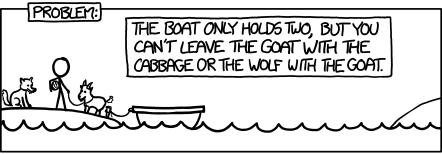
\includegraphics[scale=1]{xkcd/logic_boat_problem}}
%			\only<2|handout:2>{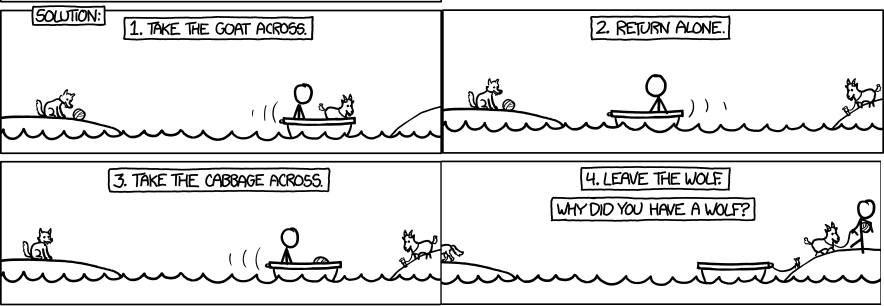
\includegraphics[scale=0.35]{xkcd/logic_boat_sol}}
%			\vspace{-2pt}
%			\url{http://xkcd.com/1134/}
%		\end{figure} 
%	}
%}

\begin{frame}{Aussagenlogik}
	Aussagen sind Sätze, die entweder \textbf{wahr} oder \textbf{falsch} sind.\\
	Deren Wahrheitswert muss dabei nicht unbedingt bekannt oder \enquote{tatsächlich ermittelbar} sein.
	
	\pause
	\begin{Beispiel}
		\begin{itemize}
			\item „$ 1 + 1 = 2 $“ ist eine Aussage. Sie ist wahr.
			\item \enquote{Es gibt nur endlich viele Primzahlen.} ist eine Aussage. Sie ist falsch.
			\pause
			\item Die Goldbachsche Vermutung (Jede gerade Zahl größer 2 ist Summe zweier Primzahlen) \pause ist eine Aussage. Ihr Wahrheitswert ist unbekannt.
			\pause
			\item „Die Welt wird am 11.11.11111 untergehen.“ \pause ist auch eine Aussage. Wir werden ihren Wahrheitswert aber wohl niemals ermitteln können.
			\pause
			\item \enquote{Gelb} ist keine Aussage.
			\pause
			\item \enquote{Dieser Satz ist falsch.} \pause ist keine Aussage. Dem Satz kann offensichtlich kein Wahrheitswert zugeordnet werden.
		\end{itemize}
	\end{Beispiel}
\end{frame}

\begin{frame}{Zwei Grundsätze der Aussagenlogik}
	
	\begin{itemize}
		\pause
		\item[1.] Jede Aussage ist \textbf{entweder} wahr \textbf{oder} falsch.\\
		Wir schreiben im Folgenden $\BB= \{\W, \F\}$
		\pause
		\item[2.] Der Wahrheitswert einer \textbf{zusammengesetzten} Aussage ist durch die
		Wahrheitswerte der \textbf{Teilaussagen} eindeutig festgelegt. \\
		\enquote{$2 + 2 = 5 \; \bimp \; \text{Pinguine können fliegen}$} ist \textbf{wahr}.\\[0.2em]
		%TODO
		%Ex falso quodlibet
	\end{itemize}

	\impl Weg vom Inhalt und betrachte stattdessen \textbf{Aussagevariablen}.
\end{frame}

\begin{frame}{Syntax}
	\begin{Definition}
		$Var_{AL}$ ist die Menge aller \textbf{Aussagevariablen}. \\
		Wir bilden aussagenlogische Formeln als Wörter über dem Alphabet $A_{AL} = \{ \bleftBr, \brightBr, \bnot, \bund, \boder, \bimp \} \cup Var_{AL}$ 
	\end{Definition}
	\pause
	\begin{Definition}
		$For_{AL}$ ist die Menge aller \textbf{syntaktisch korrekten Formeln} über $Var_{AL}$.\\
		\medskip
		(VL: induktive Definition über Konstruktionsabbildungen) \\
		Klammern, die überflüssig sind, können weg. Wir lesen es dann wie gewohnt (\enquote{$\bnot$} vor \enquote{ $\bund$} vor \enquote{ $\boder$} vor \enquote{ $\bimp$}  {\small \#PunktVorStrichUndSo}).
	\end{Definition}
	\pause
	\begin{Beispiel}
		$$Var_{AL} = \{\alA, \alB, \alC\}$$
		$$For_{AL} = \set{\alka \alA  \bimp \alB \alkz \boder \bnot \alB \bund \alC, \ \alC \bimp \alka \bnot \alC \alkz, ...}$$ 
	\end{Beispiel}
\end{frame}

\begin{frame}{Semantik}
	Die Semantik einer aussagenlogischen Formel wird durch ihre \textbf{Auswertung} bestimmt.\\
	Hierbei werden den Operatorsymbolen aus $A_{AL}$ boolesche Funktionen zugeordnet.
	
	\pause
	\begin{Definition}
		Eine \textbf{boolesche Funktion} ist eine Abbildung der Form
		$f \from \BB^n \functionto \BB$.
	\end{Definition}

	\pause
	\begin{Beispiel}
		\enquote{Handelsübliche} boolesche Funktionen sind  $b_{\bnot}$,
		$b_{\bund}$, $b_{\boder}$ und $b_{\bimp}$. 
	\end{Beispiel}
\end{frame}

\begin{frame}{Semantik}
	\let\w\W
	\let\f\F
	\begin{center}
		\begin{huge}
			$$\only<1-2|handout:1>{\bnot}\only<3-4|handout:2>{\bund}\only<5-6|handout:3>{\boder}\only<7-8|handout:4>{\bimp}$$
		\end{huge}
		Wahrheitstabelle: \\
		\medskip
		\only<1-2|handout:1>{
			\begin{tabular}{|c|c|}
				\hline 
				$A$ &  $\bnot A$ \\
				\hline
				\w & \uncover<2|handout:1>{\f} \\
				\hline
				\f & \uncover<2|handout:1>{\w} \\
				\hline
			\end{tabular}
		}
		\only<3-4|handout:2>{ 
			\begin{tabular}{|c|c|c|}
				\hline 
				$A$ & $B$ & $A \mathop{\bund} B$ \\
				\hline
				\w & \w & \uncover<4|handout:2>{\w} \\
				\hline
				\w & \f & \uncover<4|handout:2>{\f} \\
				\hline
				\f & \w & \uncover<4|handout:2>{\f} \\
				\hline
				\f & \f & \uncover<4|handout:2>{\f} \\
				\hline
			\end{tabular}
		}
		\only<5-6|handout:3>{ 
			\begin{tabular}{|c|c|c|}
				\hline 
				$A$ & $B$ & $A \mathop{\boder} B$ \\
				\hline
				\w & \w & \uncover<6|handout:3>{\w} \\
				\hline
				\w & \f & \uncover<6|handout:3>{\w} \\
				\hline
				\f & \w & \uncover<6|handout:3>{\w} \\
				\hline
				\f & \f & \uncover<6|handout:3>{\f} \\
				\hline
			\end{tabular}
		}
		\only<7-8|handout:4>{
			\begin{tabular}{|c|c|c|}
				\hline 
				$A$ & $B$ & $A \mathop{\bimp} B$ \\
				\hline
				\w & \w & \uncover<8|handout:4>{\w} \\
				\hline
				\w & \f & \uncover<8|handout:4>{\f} \\
				\hline
				\f & \w & \uncover<8|handout:4>{\w} \\
				\hline
				\f & \f & \uncover<8|handout:4>{\w} \\
				\hline
			\end{tabular}
		}
	\end{center}
\end{frame}

\begin{frame}{Semantik}
	Wenn wir den Wahrheitswert einer \textbf{zusammengesetzten} Aussage bestimmen wollen, brauchen wir die Werte der \textbf{verwendeten Aussagenvariablen}. \\
	\begin{Definition}
		Sei $V \subseteq Var_{AL}$ die Menge der verwendeten Aussagevariablen.\\
		Eine Funktion $I \from V \functionto \BB$ bezeichnet man als \textbf{Interpretation}.
	\end{Definition}
	
	

\end{frame}

\begin{frame}{Auswertung}
	\begin{Definition}
		Sei $I$ eine Interpretation. Dann liefert die Abbildung $val_I(A)$ den Wahrheitswert zu einer aussagenlogischen Formel $A$. \\
		\medskip
		Diese Funktion nennen wir \textbf{Auswertung} und berechnen sie schrittweise, z.~B.:
	\end{Definition}
	
	\begin{align*}
	&val_I(\alka\alA \bimp \alB\alkz \boder \bnot \alB)  \\
	\visible<2->{= \;&b_{\boder} (val_I(\alA\bimp \alB), val_I(\bnot \alB)) \\}
	\visible<3->{= \;&b_{\boder} (b_{\bimp} (val_I(\alA), val_I(\alB)), b_{\bnot}(val_I(\alB))) \\}
	\visible<4->{= \;&b_{\boder} (b_{\bimp} (I(\alA), I(\alB)), b_{\bnot}(I(\alB))) \\}
	\end{align*}
\end{frame}

\begin{frame}{Auswertung}
	\begin{Definition}
		Eine \textbf{Tautologie} ist eine aussagenlogische Formel, bei der für alle möglichen Interpretationen $I$ gilt: $val_I(A) = \W$. \\
		\impl Schreibweise: \quad $\models A$ \\
		\medskip
		
		\pause
		Zwei aussagenlogische Formeln $A$ und $B$ heißen \textbf{äquivalent}, wenn für jede beliebige Interpretation $I$
		$$val_I(A) = val_I(B)$$
		gilt. \\
		\impl Schreibweise: \quad $A \equiv B$
	\end{Definition}
\end{frame}

% TODO
%\begin{frame}[t]{Auswertung}
%	\only<all:1>{
\includegraphics[scale=0.65]{al_uebung_1}\\[2em]
%	Quelle: GBI-Übung 2015/2016}
%	\only<all:2>{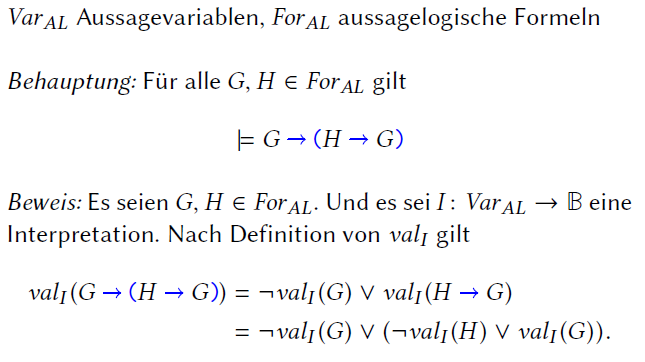
\includegraphics[scale=0.65]{al_uebung_2}}
%	\only<all:3>{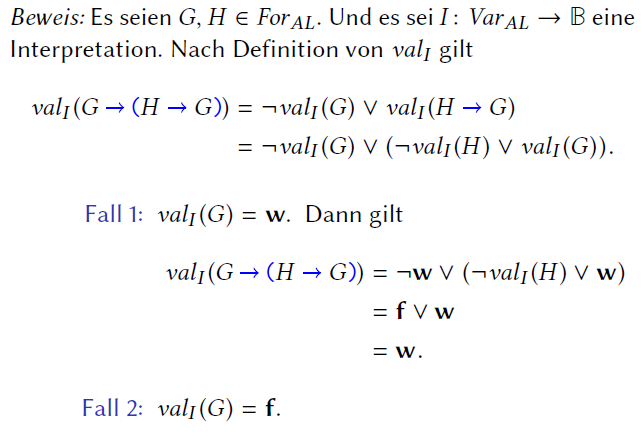
\includegraphics[scale=0.65]{al_uebung_3}}
%	\only<all:4>{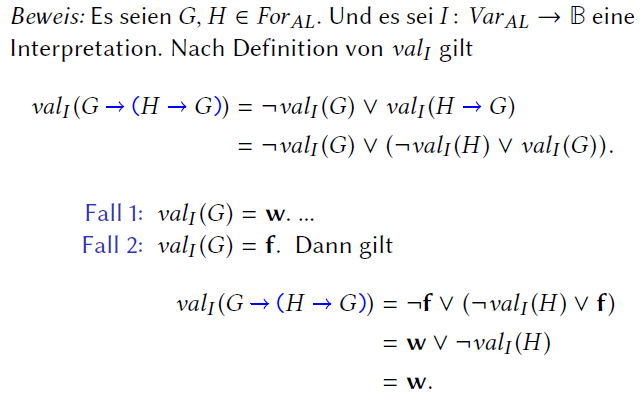
\includegraphics[scale=0.65]{al_uebung_4}}
%	\only<all:5>{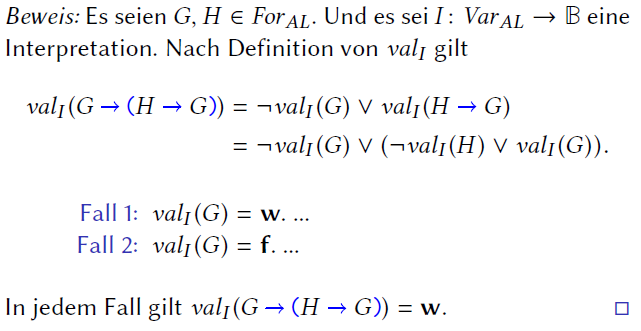
\includegraphics[scale=0.65]{al_uebung_5}}
%\end{frame}

\begin{frame}{Semantik}
	
	Möchte man eine AL-Formel für alle möglichen Interpretationen auswerten, so macht man dies meist in Form einer \textbf{Wahrheitstabelle}.
	
	\begin{block}{Aufgabe}
		Gegeben seien die Formeln
		$$ F_1 = \left(\left(\left(\alB \bimp \alA \right) \boder \alB \right) \bimp (\bnot \alA)\right) \bund \alB$$
		und
		$$F_2 = \bnot \alA \bund \alB$$
		Stellt die Wahrheitstabellen von $F_1$ und $F_2$ auf. Sind die beiden Formeln äquivalent?
	\end{block}
\end{frame}

\begin{frame}{Lösung}
	Für die Formel $F_1$:
	\begin{table}[H]
	\centering
	\begin{tabular}{|*{6}{c|}}
	\hline
	$\alA$ & $\alB$ & $\alB \bimp \alA$ &  $\dots \boder \alB$ & $\dots \bimp \bnot \alA$ & $\dots \bund \alB$ \pause \\ \hline
	\W & \W & \W & \W & \F & \F  \\ \hline \pause
	\W &  \F & \W & \W & \F & \F  \\ \hline \pause
	\F & \W & \F & \W & \W & \W  \\ \hline \pause
	\F & \F & \W & \W & \W & \F \\ \hline
	\end{tabular}
	\end{table}
\end{frame}

\begin{frame}{Lösung}
	Für die Formel $F_2$:
	\begin{table}[h!]
	\centering
	\begin{tabular}{|*{3}{c|}}
	\hline
	$\alA$ & $\alB$ & $\bnot \alA \bund \alB$  \\ \hline \pause
	\W & \W & \F \\  \hline \pause
	\W & \F & \F \\  \hline \pause
	\F & \W & \W \\  \hline \pause
	\F & \F & \F \\ \hline
	\end{tabular}
	\end{table}
	Also sind die beiden Formeln äquivalent: $$F_1 \equiv F_2$$
\end{frame}


\input{../Bloecke/Aussagenlogik2}

\section{Formale Sprachen}

\begin{frame}{Rückblick}
	Sei $A = \{\word A, \word B, ..., \word Z, \word a, \word b, ..., \word z, \word\sp\}$ ein Alphabet.\\
	\pause
	Dann enthält $A^*$ alle Wörter, die man mit Zeichen aus $A$ bilden kann. Aber nicht jedes dieser Wörter ist auch sinnvoll.\\[1em]
	
	\enquote{\word{\thassedaniel{egnarts\sp si\sp efiL}{retsinnaL\sp nosrO}}} ist kein sinnvolles Wort. \pause Oder? \\[1em]
	\pause
	\impl Hängt vom Kontext ab!\\
	
\end{frame}

\begin{frame}{Formale Sprachen}
		\begin{Definition}
			Sei $A$ ein Alphabet.\\
			Eine \textbf{formale Sprache} $L$ ist eine Teilmenge von $A^*$.
		\end{Definition}
		\pause
		\vspace{10pt}
		Durch eine formale Sprache geben wir an, welche der möglichen Wörter über $A$ wir in einem bestimmten Kontext als „wünschenswert“/„interessant“ ansehen.\\
		\pause \smallskip
		Formale Sprachen werden häufig nicht direkt, sondern über Bildungsvorschriften angegeben.
		
		\pause
		\begin{Beispiel}
			$A = \{\word 0, \word 1\}$ \\
			$L = \{ w \in A^* \mid w \text{ endet auf } \word{10} \}  = \{\word{10}, \word{010}, \word{110}, \word{0010}, ...\}$
		\end{Beispiel}
\end{frame}







\begin{frame}{Produkt}
		\begin{Definition}
			Seien $L_1$ und $L_2$ zwei formale Sprachen. Dann bezeichnet
				$$L_1 \cdot L_2 := \{w_1 w_2 \mid w_1 \in L_1 \text{ und } w_2 \in L_2 \}$$
				das \textbf{Produkt} der Sprachen $L_1$ und $L_2$.
		\end{Definition}
		\pause
		In $L_1 \cdot L_2$ sind also alle Wörter enthalten, deren erster Teil aus $L_1$ und deren zweiter Teil aus $L_2$ ist.
	
\end{frame}

\begin{frame}{Produkt}
	\begin{Beispiele}
		$\{\word a, \word b\} \cdot \{\word c, \word d\} = \{\word{ac}, \word{ad}, \word{bc}, \word{bd}\}$\\[0.3em]
		\pause
		$ L = \{w_1w_2 \mid w_1\in \{\literal{b}\}^* ,  w_2\in \{\literal{a}\}^* \} 
		= \{\literal{b}\}^* \cdot \{\literal{a}\}^* $\\[1em]
		\pause
		Für alle formalen Sprachen $L$ gilt:\\
		$$ L \cdot \{\varepsilon\} = L  \qquad L \cdot \emptyset = \emptyset$$
	\end{Beispiele}
\end{frame}



\begin{frame}{Potenzen}
	\begin{Definition}
	Potenzen formaler Sprachen definieren wir induktiv so: 
	$$L^0 := \{\varepsilon \}$$
	$$L^{i+1} := L^i \cdot L$$
	\end{Definition} \pause
	$L^i$ enthält also alle Kombinationen von $i$ (nicht unbedingt verschiedenen) Wörtern aus $L$.
\end{frame}

\begin{frame}{Konkatenationsabschluss}
	\begin{Definition}
		Der \textbf{Konkatenationsabschluss} einer Sprache $L$ ist \quad $L^\ast = \bigcup \limits_{i=0}^\infty L^i$. \\
		$$ \set{}^* = \set{ \eps } \qquad \set{\word{abc}, \word{xy}}^* = \set{\eps, \word{abc}, \word{xy}, \word{abcabc}, \word{abcabcxy}, \word{xyabc}, ...} $$ 
		\medskip
		\pause
		Der \textbf{$\eps$-freie Konkatenationsabschluss} ist \quad $L^+ = \bigcup \limits_{i=1}^\infty L^i$. \\
		$$ \set{}^+ = \set{} \qquad \set{\word{abc}, \word{xy}}^+ = \set{\word{abc}, \word{xy}, \word{abcabc}, \word{abcabcxy}, \word{xyabc}, ...} $$
	\end{Definition} \pause
	\textbf{Achtung}: Der $\eps$-freie Konkatenationsabschluss muss nicht „$\eps$-frei“ sein! \\ \pause
	$$ \set{\eps}^+ = \underbrace{\set{\eps}}_{\mathclap{\text{enthält ein $\eps$!}}} $$
	
\end{frame}

\begin{frame}{Beispiele aus dem Leben}
	\begin{itemize}
		\item Sprache der korrekten IP4-Adressen: \pause
		\begin{align*}
		\set{\word{192.168.178.1}, \quad 
			\word{76.147.112.6}, ... }
		\end{align*} 
		\pause Enthält aber nicht: $\word{000.999.123.666}$ \pause
		\item Formale Sprache der Schlüsselwörter in Java: $$L = \{ \word{class}, \word{int} , \word{if}, \dots \}$$ \pause
		\item Formale Sprache der ganzen Zahlen: Mit $A = \{\word 0, ..., \word 9\}$ bauen wir
		\pause $$A \cdot A^* = \{\word{12849}, \word{1001}, \word{42}, ...\}$$ 
		\pause Und minus? Also besser $ \{ \mword-, \varepsilon \} \cdot A \cdot A^*$
	\end{itemize}
\end{frame}

\begin{frame}{Formale Sprachen}
	
	\begin{Beispiel}
		Sei $L$ formale Sprache aller Wörter über $A=\{\literal{a},\literal{b}\}$, in denen nirgends das Teilwort $\literal{ab}$ vorkommt.
		\begin{itemize}
			\pause
			\implitem $L=\{\literal{a},\literal{b}\}^*
			\setminus \set{w_1 \cdot \literal{ab} \cdot w_2 \mid w_1,w_2\in
			\{\literal{a},\literal{b}\}^* }$
			
			\pause
			\item Erst ein beliebiges Wort (evtl. $\varepsilon$) nur aus $\literal{b}$,\\
			danach ein beliebiges Wort (evtl. $\varepsilon$) nur aus $\literal{a}$.
			
			\pause
			\implitem $L=\set{w_1w_2 \mid w_1\in 
			\{\literal{b}\}^*  \text{ und }  w_2\in \{\literal{a}\}^* }$
		\end{itemize}
	\end{Beispiel}
	
	\begin{block}{Bemerkungen}
		\begin{itemize}
			\pause
			\item Die Beschreibung einer formalen Sprache ist \textbf{nicht} eindeutig (siehe oben).
			\pause
			\item Immer auf den Unterschied achten: $\{\literal{abc} \} \neq \literal{abc} $
		\end{itemize}
	\end{block}
\end{frame}


\begin{frame}{Aufgabe}
	Es sei $A = \{\word a, \word b\}$. Beschreibt die folgenden formalen Sprachen mit den Symbolen $\word\{, \word\}, \word a, \word b, \textcolor{blue}{\eps}, 
	\mword{\cup}, 
	\mword{{}^*}, \mword{{}^+},
	\word, , \mword{\cdot} , \word( \text{ und } 
	\word)
	$:
	\begin{itemize}
		\item die Menge aller Wörter über $A$, die das Teilwort \word{ab} enthalten. \\
		\uncover<2-|handout:2>{$\{\word a, \word b\}^\ast \cdot \{\word{ab}\} \cdot \{\word a, \word b\}^\ast$}
		\item die Menge aller Wörter über $A$, deren vorletztes Zeichen ein \word b ist. \\
		\uncover<3-|handout:2>{$\{\word a, \word b\}^\ast \cdot \{\word b\} \cdot \{\word a, \word b\}$}
		% $\{\word a, \word b\}^\ast \cdot \{\word b\} \cdot \{\word a, \word b\}$
		\item die Menge aller Wörter über $A$, in denen nirgends zwei \word bs unmittelbar hintereinander vorkommen. \\
		\uncover<4-|handout:2>{$\{\word a, \word{ba}\}^\ast \cdot \{ \word b, \eps \}$}
	\end{itemize}
\end{frame}




\mycomment{
	\section{Sprachen: Aufwärmen}
	
	
	\begin{frame}{Rückblick}
		\begin{itemize}
			\item \textbf{Alphabet} $A$ mit Zeichen, aus denen wir Wörter zusammenbauen
			\item Nicht immer haben all diese Wörter einen Sinn
			\item Wir definieren selbst, welche Wörter wir als korrekt ansehen und akzeptieren wollen.
			\item Eine solche Teilmenge aller möglichen Wörter nennen wir \textbf{formale Sprache}
		\end{itemize}
	\end{frame}
}




% TODO: Im letzten Jahr hat die Zeit nicht gereicht,
% daher diesen Inhalt hier eher streichen.
%\def\mycircle{\raisebox{1pt}{\Circle}}

\morescalingdelimiters

\section{Sprache gesucht}

\begin{frame}{Sprache gesucht!} 
	Haben Alphabet $A = \{ \mword \triangle, \mword \square, \mword \mycircle \}$.\\
\end{frame}

%\begin{frame}
%	\frametitle{Zum Aufwärmen: Sprache gesucht!}
%	
%	Ihr erhaltet eine Karte mit einer Beschreibung einer formalen Sprache über dem Alphabet $\Sigma = \{ \triangle, \square, \circ \}$.\\
%	Ziel ist es, jeweils alle Beschreibungen von gleichen Sprachen zu sammeln.\\
%	Dazu überlegt ihr euch zunächst in 4er-Gruppen, ob ihr Beschreibungen von gleichen Sprachen habt oder was andere Beschreibungen wären. \\
%	Dann tauschen sich jeweils 3 4er-Gruppen aus und sammeln die Beschreibungen.
%\end{frame}

\begin{frame}{Sprache gesucht!}
	
	Die Sprache der Wörter, die mit einem Kreis beginnen und danach keinen Kreis mehr enthalten.
	\bigskip
	\pause
	
	$$ \{\mword \mycircle\} \cdot \{\mword \triangle, \mword \square\}^* $$
	\bigskip
	\pause
	
	$$ \set{w \in A^* \mid w = \mword \Circle \cdot v, v \in \{\mword \triangle, \mword \square\}^* } $$

\end{frame}

\begin{frame}{Sprache gesucht!}
	
	Die Sprache der Wörter, deren vorletztes Zeichen ein Dreieck ist.
	\bigskip
	\pause
	
	$$ \{\mword \triangle, \mword \square, \mword \mycircle\}^* \cdot \set{\mword \triangle} \cdot \{\mword \triangle, \mword \square, \mword \mycircle\} $$
	\bigskip
	\pause

	$$ \{w \in A^* \mid w = v \cdot \mword \triangle \cdot z, v \in A^*, z \in A \} $$

	
\end{frame}

\begin{frame}{Sprache gesucht!}
	Die Sprache der Wörter, in denen nirgends eine ungerade Anzahl an Dreiecken nebeneinander steht.
	\bigskip
	\pause
	$$ \left(\{\mword \square, \mword \mycircle\}^* \cdot \{\mword \triangle\mword \triangle\}^* \right)^* $$
\end{frame}

\begin{frame}{Sprache gesucht!}
	
	
	Die Sprache der Wörter, in denen eine gerade Anzahl an Vierecken vorkommt.
	\bigskip
	\pause
	$$ \{\mword \triangle, \mword \mycircle\}^* \cdot \left( \{\mword \square\} \cdot \{\mword \triangle, \mword \mycircle\}^* \cdot \{\mword \square\} \cdot \{\mword \triangle, \mword \mycircle\}^* \right)^* $$
	

\end{frame}

\begin{frame}{Sprache gesucht!}
	Die Sprache der Wörter, in denen nirgends zwei Kreise aufeinander folgen.
	\bigskip
	\pause
	$$ \{\mword \square, \mword \triangle\}^* \cdot \left( \{\mword \mycircle\} \cdot \{\mword \square, \mword \triangle\}^+ \right)^* \cdot \{\mword \mycircle, \varepsilon\} $$
	

	
\end{frame}

\section{Mehr zu formalen Sprachen}

\begin{frame}{Beispiel}
	Sei $A = \set{\word a,\word b}$ ein Alphabet. Mit $L$ wollen wir alle Wörter beschreiben, die genau ein $\word b$ enthalten. \\ \pause
	$$ L = \set{w_1 \word b w_2 \mid w_1, w_2 \in \{\word a\}^\ast } = \{\word a\}^\ast \cdot \{\word b \} \cdot \{\word a\}^\ast$$
	
	Was ist $L^3$? Was enthält $L^i$? \pause
	Zum Beispiel ist $$\word{aaababaaaabaa} = \word{aaaba} \cdot \word{baa} \cdot \word{aabaa} \in L_3$$ \pause
	$L^i$ enthält alle Wörter, die genau $i$-mal ein \word b enthalten! \\[1em]
	
	Was enthält $$L^i \setminus \{\word b\}^\ast ?$$ \pause
	Alle Wörter, die aus $i$ \word bs bestehen, aber auch noch mindestens ein \word a enthalten. \\
\end{frame}

\begin{frame}{Aufgabe}
	Welche Eigenschaft muss eine formale Sprache $L$ über einem Alphabet
	$A$ erfüllen, damit gilt: $$ L^0 \subseteq L^1 \subseteq L^2 \subseteq L^3 \subseteq ... $$
	
	\pause
	\begin{block}{Lösung}
		Das gilt, wenn $$ \varepsilon \in L $$
	\end{block}
	
\end{frame}

\subsubsection{A1}
\begin{frame}{Aufgabe (Klausur)}
		\begin{itemize}
			\item[(1)] Widerlegt: Für alle formalen Sprachen $L_1 , L_2$ gilt: 
			$$L_1^\ast \cup L_2^\ast = (L_1 \cup L_2 )^\ast$$
			
			\item[(2)] Zeigt: Für alle formalen Sprachen $L$ gilt: 
				$$L^\ast \cdot L = L^+ $$ 
	\end{itemize}

	Tipp zu (2) (nicht in der Klausur gegeben): Hier handelt es sich um eine Mengengleichheit, also brav mit \enquote{$\subseteq$} und \enquote{$\supseteq$} beweisen! \smiley 
\end{frame}

\begin{frame}[t]{Lösung}
	\textit{Für alle formalen Sprachen $L_1 , L_2$ gilt: 
		$$L_1^\ast \cup L_2^\ast = (L_1 \cup L_2 )^\ast$$ } \\[2em] \pause
	Diese Aussage ist falsch: Sei $L_1 = \{\word a\}$ und $L_2 = \{\word b\}$. Dann liegt \word {ab} in $(L_1 \cup L_2 )^\ast = \{\word a, \word b\}^\ast$ aber nicht in $L_1^\ast \cup L_2^\ast = \{\word a\}^\ast \cup \{\word b\}^\ast$.
\end{frame}

\begin{frame}[t]{Lösung}
	\textit{Für alle formalen Sprachen $L$ gilt: 
		$$L^\ast \cdot L = L^+ $$ } \\[1em] \pause
	Diese Aussage ist wahr! 
	\begin{block}{1. Schritt: $L^\ast \cdot L \subseteq L^+$:} \pause
	Wenn $w \in L^\ast \cdot L$ liegt, dann lässt es sich in Teilwörter auftrennen $$ w = w_1 \cdot w_2$$ mit $w_1 \in L^\ast$ und $w_2 \in L$. Für $w_1$ existiert ein $i \in \N_0$ mit $w_1 \in L^i$. Also $$w = w_1 w_2 \in L^i \cdot L = L^{i+1} \subset L^+.$$
	\end{block}
\end{frame}

\begin{frame}[t]{Lösung}
	\textit{Für alle formalen Sprachen $L$ gilt: 
		$$L^\ast \cdot L = L^+ $$ } \\[1em] 
	Diese Aussage ist wahr! 
	\begin{block}{2. Schritt: $L^\ast \cdot L \supseteq L^+$:} \pause
	Wähle nun $w \in L^+$. Dann existiert ein $i \in \N_+$ mit $w \in L^i$. Da $i > 0$ lässt es sich schreiben als $i = j + 1$ für ein $j \in \N_0$. Also ist $$w \in L^{j+1} = L^j \cdot L \subset L^\ast \cdot L. \qed$$
	\end{block}
\end{frame}

\subsubsection{A2}
\begin{frame}{Aufgabe (WS 2008)}
	Es sei $A = \{\word a, \word b\}$. Die Sprache $L \subset A^\ast$ sei definiert durch $$L = \left(\{\word a\}^\ast \cdot \{\word b\} \cdot \{\word a\}^\ast \right)^\ast$$
	Zeigt, dass jedes Wort $w$ aus $\{\word a, \word b\}^\ast$, das mindestens einmal das Zeichen
	\word b enthält, in $L$ liegt. (Hinweis: Macht eine Induktion über die Anzahl der
	Vorkommen des Zeichens \word b in $w$.)
\end{frame}

\begin{frame}{Lösung}
	$$L = \left(\{\word a\}^\ast \cdot \{\word b\} \cdot \{\word a\}^\ast \right)^\ast$$
	Sei $k$ die Anzahl der Vorkommen von \word b in einem Wort $w \in \{\word a, \word b\}^\ast$.
	\begin{block}{Induktionsanfang}  \pause
		Für $k = 1$: In diesem Fall lässt sich das Wort $w$ aufteilen in $$w = w_1 \cdot \word b \cdot w_2$$ wobei $w_1$ und $w_2$ keine \word b enthalten und somit in $\{\word a\}^\ast$ liegen. Damit gilt $w \in \{\word a\}^\ast \cdot \{\word b\} \cdot \{\word a\}^\ast$ und somit auch $$w \in \left(\{\word a\}^\ast \cdot \{\word b\} \cdot \{\word a\}^\ast \right)^\ast = L$$
	\end{block}
\end{frame}

\begin{frame}{Lösung}
	\begin{block}{Induktionsvoraussetzung}  \pause
		Für ein festes $k \in \N$ gilt, dass alle Wörter über $\{\word a, \word b\}^\ast$, die genau $k$-mal das Zeichen \word b enthalten, in $L$ liegen.
	\end{block} \pause
	\begin{block}{Induktionsschritt}  \pause
		Wir betrachten ein Wort $w$, das genau $k + 1$ mal das Zeichen \word b enthält. Dann kann man $w$ zerlegen in $w = w_1 \cdot w_2$, wobei $w_1$ genau einmal das Zeichen \word b enthält und $w_2$ genau $k$-mal das Zeichen \word b. \pause Nach Induktionsanfang liegt $w_1$ in $\{\word a\}^\ast \{\word b\}\{\word a\}^\ast$. Nach Induktionsvoraussetzung liegt $w_2$ in $(\{\word a\}^\ast \{\word b\}\{\word a\}^\ast )^\ast$, was bedeutet, dass $w = w_1 \cdot w_2$ in $$\left(\{\word a\}^\ast \{\word b\}\{\word a\}^\ast \right) \* \left(\{\word a\}^\ast \{\word b\}\{\word a\}^\ast \right)^\ast \subseteq \left(\{\word a\}^\ast \{\word b\}\{\word a\}^\ast \right)^\ast = L$$ liegt und die Behauptung ist gezeigt. $\qed$
	\end{block}
\end{frame}

%\subsubsection{A3}
%\begin{frame}
%	\frametitle{Noch mehr Aufgaben}
%	Begründen oder widerlegen Sie:
%	\begin{itemize}
%		\item Für alle formalen Sprachen $L$ gilt: 
%		$$(L_1^\ast \cdot L_2^\ast)^\ast = (L_1 \cdot L_2)^\ast$$ 
%		
%		\item Für alle formalen Sprachen $L_1 , L_2$ gilt: 
%		$$(L_1^\ast \cup L_2^\ast)^\ast = (L_1 \cup L_2 )^\ast$$
%	\end{itemize}
%\end{frame}
%
%\begin{frame}
%	\frametitle{Lösung}
%	\textit{Für alle formalen Sprachen $L_1 , L_2$ gilt: 
%		$$(L_1^\ast \cdot L_2^\ast )^\ast = (L_1 \cdot L_2 )^\ast$$ } \\[2em] \pause
%	Diese Aussage ist falsch: Sei $L_1 = \{a\}$ und $L_2 = \{b\}$. Dann liegt $$\mathbf{aa} = \mathbf{aa} \cdot \varepsilon$$ in $(L_1^\ast \cdot L_2^\ast ) = (L_1^\ast \cdot L_2^\ast )^1 \subset (L_1^\ast \cdot L_2^\ast )^\ast$, aber nicht in $(L_1 \cdot L_2 )^\ast = \{ab\}^\ast$.
%	
%\end{frame}
%
%\begin{frame}
%	\frametitle{Lösung}
%	\textit{Für alle formalen Sprachen $L_1 , L_2$ gilt: 
%		$$(L_1^\ast \cup L_2^\ast )^\ast = (L_1 \cup L_2 )^\ast$$ } \\[2em] \pause
%	Die Aussage ist korrekt: Sei $w$ ein Wort aus $(L_1^\ast \cup L_2^\ast )^\ast$. Dieses lässt sich in Teilwörter $w_1 , \cdots , w_k$ unterteilen, so dass für $1 \leq i \leq k$ gilt: 
%	$$w_i \in (L_1^\ast \cup L_2^\ast ) \implies w_i \in L_1^\ast \text{ oder } w_i \in L_2^\ast$$
%	Diese Teilwörter $w_i$ lassen sich wieder in Teilwörter $w_{i_1}, \dots w_{i_s}$ zerlegen, die entweder aus $L_1$ kommen, wenn $w_i \in L_1^\ast$ liegt, oder in $L_2$ liegen, wenn $w_i \in L_2^\ast$ liegt. Damit lässt sich $w$ in Teilwörter $w_{i_j}$ aus $L_1 \cup L_2$ unterteilen und es folgt $w \in (L_1 \cup L_2 )^\ast$. 
%\end{frame}
%
%\begin{frame}
%	\frametitle{Lösung}
%	\textit{Für alle formalen Sprachen $L_1 , L_2$ gilt: 
%		$$(L_1^\ast \cup L_2^\ast )^\ast = (L_1 \cup L_2 )^\ast$$ } \\[2em]
%	Sei umgekehrt ein Wort $w$ aus $(L_1 \cup L_2 )^\ast$. Dieses lässt sich dann in Teilwörter $w_1, \dots, w_k$ unterteilen, so dass für $1 \leq i \leq k$ gilt 
%	$$w_i \in L_1 \cup L_2 \implies w_i \in L_1 \subset L_1^\ast \text{ oder } w_i \in L_2 \subset L_2^\ast$$
%	Somit lässt sich $w$ in Teilwörter aus $L_1^\ast \cup L_2^\ast$ unterteilen, und es folgt $w \in (L_1^\ast \cup L_2^\ast )^\ast$.
%\end{frame}

\begin{frame}{Ausblick: Klammerausdrücke}
	
	Was ist mit der Sprache aller gültigen Klammerausdrücke? Können wir die auch mit $\set{}$, $\*$, ${}^*$ und ${}^+$ angeben? \only<beamer:0>{\\ \emph{Spoiler: Nein, das geht nicht!}}\\[1em]
	\pause
	
	\begin{block}{}
		\Large
		\centering
		COMING SOON... \\[1em]
	\end{block}

	\begin{figure}[H]
		\centering
		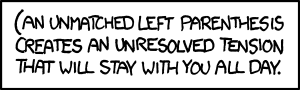
\includegraphics[scale=0.7]{xkcd/(.png}
		\vspace{-7pt}
		\caption{ \texttt{\url{https://xkcd.com/859/}} }
	\end{figure}
\end{frame}

%\section{Von der Darstellung zur Zahl}

\subsection{Definitionen}
\begin{frame}{Numerischer Wert einer Ziffernfolge}
	\begin{Definition}
		Zu einer Zahlenbasis $b$ definiere 
		\begin{align*}
			\fnum_b &\from Z_b \functionto \Z \\
			\fnum_b(x) &:= x \text{ (als Zahl)} \quad \text{für einzelne Ziffern $x \in Z_b$} \\
			& \\
			\fNum_b &\from Z_b^* \functionto \Z \\
			\fNum_b(\eps) &:= 0 \\
			\fNum_b(wx) &:= b\cdot \fNum_b(w) + \fnum_b(x) \quad \text{ für alle } w\in Z_b^\ast, x\in Z_b. 
		\end{align*}
	\end{Definition}

	\pause
	\textbf{Hinweis}: $\fNum_b$ ist eine Abbildung, die einem Wort (Zahlendarstellung) eine Zahl (Wert) zuordnet. \\
	Wir schreiben für die Zahl aber wieder eine Darstellung hin (nämlich im Dezimalsystem).
\end{frame}
\begin{frame}{Aufgabe}
	Berechnet die Zahlenwerte von $ \word{11}_2, \word{321}_4, \word{B2}_{16}$.
	\begin{align*} 
	\fNum_2(\word{11}) &= \visible<2->{2\cdot \fNum_2(\word 1) + \fnum_2(\word 1) \\
	&= 2\cdot 1 + 1 \\
	&= 3  \\}
	\visible<3->{\fNum_4(\word{321}) &=} \visible<4->{ 4\cdot \fNum_4(\word{32}) + \fnum_4(\word 1) \\
	&= 4\cdot \left( 4\cdot \fNum_4(\word 3) + \fnum_4(\word 2) \right) + \fnum_4(\word 1) \\
	&= 4^2\cdot \fnum_4(\word 3) + 4 \cdot \fnum_4(\word 2) + \fnum_4(\word 1) \\
	&= 57 \\}
	\visible<5->{\fNum_{16}(\word{B2}) &=} \visible<6->{ 16 \cdot \fNum_{16}(\word B) + \fnum_{16}(\word 2) \\
	&= 16\cdot 11 + 2 \\
	&= 178}
	\end{align*}

\end{frame}

\mycomment{  % man sieht hier nicht viel...
	\begin{frame}{Wohldefiniertheit}
		\emph{Behauptung}: Die Definition 
			$$ \fNum_b(\eps) = 0  $$  
			$$ \fNum_b(wx) = b\cdot \fNum_b(w) + \fnum_b(x) \text{ für alle } w\in Z_b^\ast, x\in Z_b $$ 
			ist wohldefiniert und weist jedem Wort eine eindeutige Bedeutung zu, die dem Zahlenwert entspricht.
	\end{frame}
	\begin{frame}{Beweis}
		\begin{block}{Beweis durch vollständige Induktion über $n=\vert w \vert $}
		\begin{itemize}
			\only<1-2>{\item<1->[{IA.:}] $n = 0 = \vert w \vert \implies w = \eps $. \\
			Für $w = \eps $ ist $\fNum_b$ wohldefiniert und sinnvoll (nämlich $\fNum_b(\eps) = 0$).
			\item<2->[{IV.:}] Für ein beliebig aber festes $n\in\N_0$ sei $\fNum_b(w)$ für alle $w$ mit $\setsize{w} = n$ wohldefiniert und entspreche dem Zahlenwert. }
			\only<3->{\item<3->[{IS.:}] Wähle $w'$ mit $\vert w' \vert = n+1 $, dann gibt es ein $w\in Z_b^n, x\in Z_b$, so dass $ w' = wx $ \\
			Mit der Definition gilt nun $$ \fNum_b(w') = b\cdot {\underbrace{\fNum_b(w)}_{IV}} + \fnum_b(x) $$
			Die Summe ist laut $IV$ wohldefiniert. Auch ist laut $IV$ $\fNum_b(w)$ der Zahlenwert von $w$ und damit auch $\fNum_b(w')$.}
		\end{itemize}
		\end{block}
	
	\end{frame}
}

%\subsection{Aufgabe}
%\begin{frame}{Aufgabe. WS 2010 }
%Es bezeichne $\Z$ die Menge der ganzen Zahlen. Gegeben sei eine Ziffernmenge $Z_{-2} = \{N, E\}$ mit der Festlegung $num_2 (N) = 0$ und $num_2 (E) = 1$. Wir definieren eine Abbildung $\fNum_{-2} : Z_{-2}^\ast \functionto \Z$ wie folgt:
%	$$\fNum_{-2} (\eps) = 0$$
%	$$\forall \ w \in Z_{-2}^\ast \ \forall \ x \in Z_{-2} : \fNum_{-2} (wx) = -2 \cdot \fNum_{-2} (w) + num_2 ( x )$$
%
%	\begin{itemize}	
%		\item Geben Sie für $w \in \{E, EN, EE, ENE, EEN, EEE\}$ jeweils $\fNum_{-2} (w)$ an.
%		\item Für welche Zahlen $x \in \Z$ gibt es ein $w \in Z_{-2}^\ast$ mit $\fNum_{-2} (w) = x$?
%	\end{itemize}
%\end{frame}
%
%\begin{frame}{Lösung}
%\textit{Geben Sie für $w \in \{E, EN, EE, ENE, EEN, EEE\}$ jeweils $\fNum_{-2} (w)$ an.} \pause
%	\begin{table}[h!]	
%		\begin{tabular}{>{$}l<{$}>{$}l<{$}}
%			\fNum_{-2} (E)\pause & = 1 \\ \pause 
%			\fNum_{-2} (EN)\pause & = -2 \\ \pause
%			\fNum_{-2} (EE)\pause & = -1 \\ \pause
%			\fNum_{-2} (ENE)\pause & = 5 \\ \pause
%			\fNum_{-2} (EEN)\pause & = 2 \\ \pause
%			\fNum_{-2} (EEE)\pause & = 3
%	\end{tabular}
%	\end{table}
%	\pause
%	\textit{Für welche Zahlen $x \in \Z$ gibt es ein $w \in Z_{-2}^\ast$ mit $\fNum_{-2} (w) = x$?} \\[1em]\pause
%	Für alle!
%\end{frame}

\section{Von der Zahl zur Darstellung}
\begin{frame}{Division und Modulo}
	\begin{block}{Definition}
		$ x \div y$ ist die ganzzahlige Division von x durch y.\\
		$ x \mod y$ liefert den Rest dieser Division.
	\end{block} 
	\pause
	
	\begin{block}{Beobachtung}
		$ x\div y \in \N_0, \qquad x\mod y \in \{0,\dots, y-1\} $
	\end{block}
	\pause
	
	\begin{Beispiel}
		\begin{tabular}{c|cccc|cccc}
			$y$ & \multicolumn{4}{c|}{2} & \multicolumn{4}{c}{3} \\
			$x$ & 1 & 2 & 5 & 8 & 1 & 2 & 5 & 8 \\ \pause
			$x\div y$ & 0 & 1 & 2 & 4 & 0 & 0 & 1 & 2 \\
			$x\mod y$ & 1 & 0 & 1 & 0 & 1 & 2 & 2 & 2 \\
		\end{tabular}
	\end{Beispiel}
	
\end{frame}

\begin{frame}{Division und Modulo}

	\begin{block}{Lemma}
		$$ x = y \cdot (x \div y ) + \left( x \mod y \right)$$ 
	\end{block}

	\begin{Beispiel}
		Für $y = 4$: \\
		\begin{table}[h!]
			\centering
			\begin{tabular}{c|cccccccccccc}
				$x$ & 0 & 1 & 2 & 3 & 4 & 5 & 6 & 7 & 8 & 9 & 10 & 11 \\ 
				\hline
				$x\div 4 $ & \only<2->{0 & 0 & 0 & 0 & 1 & 1 & 1 & 1 & 2 & 2 & 2 & 2 } \only<1|handout:0>{&&&&&&&&&&&} \\
				$4 \* \left( x\div 4\right) $ & \only<3->{0&0&0&0&4&4&4&4&8&8&8&8} \only<1-2|handout:0>{&&&&&&&&&&}  \\ 
				$x\mod 4$ & \only<4->{0&1&2&3&0&1&2&3&0&1&2&3} \only<1-3|handout:0>{&} \\
				\hline
				$4 \* \left( x\div 4\right) + x \mod 4 $ & \only<5->{0 & 1 & 2 & 3 & 4 & 5 & 6 & 7 & 8 & 9 & 10 & 11} \only<1-4|handout:0>{&&&&&&&&&&}
			\end{tabular}
		\end{table}
	\end{Beispiel}

	% \visible<5-> {$ \Impl$ \enquote{Beweis durch Beispiel} :P \qed}  % Too misleading. Mündlich ok.

\end{frame}

\begin{frame}{Repräsentation von Zahlen}
	Wir definieren
	\begin{threealign}
	\fRepr_k \from \; \N_0 &\functionto& Z_k^*,  \\
	n &\mapsto& \begin{cases} \frepr_k(n), & n<k \\ \fRepr_k\left( n\div k \right) \cdot \frepr_k\left( n \mod k \right), & n\geq k 
	\end{cases}.
	\end{threealign}
	\pause
	\begin{block}{Es gilt}
		$\fRepr_k(n)$ ist das kürzeste Wort $w\in Z_k^\ast$ mit $\fNum_k(w)=n$, also 
		$$ \fNum_k\left( \fRepr_k(n)\right) = n. $$ 
	\end{block}
	\pause
	\emph{Anmerkung}:
	Im Allgemeinen ist $$ \fRepr_k\left(\fNum_k(w)\right) \neq w, $$ da überflüssige Nullen in $w$ wegfallen können. 
\end{frame}

\begin{frame}{Exkurs: Euklid-Schema / Horner-Schema}
	\def\r{\text{ Rest }}
	\only<all:1>{
		\begin{block}{Euklid-Schema}
			\textcolor{blue}{Größte \enquote{noch reinpassende} Potenz} ermitteln. Dann durch alle absteigenden Potenzen teilen, \textbf{Ganzzahlteil} ergibt Ziffern. \underline{Rest} wird jeweils in die nächste Zeile übernommen. \\
			Beispiel: \quad $29_{10} = ???_3$
			\begin{align*}
				\text{Es gilt: } \quad \color{blue}{3^3} &\leq 29 < 3^4 \\
				{\Impl} 29 : \color{blue}{3^3} &= \textbf{1} \r \underline{2} \\
				\underline{2} : 3^2 &= \textbf{0} \r \underline{2} \\
				\underline{2} : 3^1 &= \textbf{0} \r \underline{2} \\
				\underline{2} : 3^0 &= \textbf{2} \r 0 
			\end{align*}
			\Impl $29_{10} = 1002_3$
		\end{block}
	}
	\only<all:2->{
		\begin{block}{Horner-Schema}
			Durch die Ziel-Basis teilen, Rest ergibt Ziffern \textbf{rückwärts}. \\
			\begin{align*}
				29 : 3 	 &= \underline{9} \r \textbf{2} \\
				\underline{9} : 3 &= \underline{3} \r \textbf{0} \\
				\underline{3} : 3 &= \underline{1} \r \textbf{0} \\
				\underline{1} : 3 &= 0 \r \textbf{1} 
			\end{align*}
			\Impl $29_{10} = 1002_3$ \quad (die Reste rückwärts!)
		\end{block} \only<+>{} \pause \medskip
		\Impl $\fRepr_k$ implementiert genau das Horner-Schema! \smiley
	}
\end{frame}

\begin{frame}{Repräsentation von Zahlen}
	\begin{threealign}
	\fRepr_k : \; \N_0 &\functionto& Z_k^*,  \\
	n &\mapsto& \begin{cases} \frepr_k(n), & n<k \\ \fRepr_k\left( n\div k \right) \cdot \frepr_k\left( n \mod k \right), & n\geq k 
	\end{cases}
	\end{threealign}
	
	\begin{block}{Aufgabe}
		Berechnet folgende Darstellungen mit dem Horner-Schema:\\
		$\fRepr_2(42) = \only<2->{\word{101010}}$ \\
		$\fRepr_4(42) = \only<3->{\word{222}}$ \\
		$\fRepr_8(42) = \only<4->{\word{52}}$ \\
		$\fRepr_{16}(42) = \only<5->{\word{2A}}$
	\end{block}
\end{frame}

\begin{frame}{Beispiel: ausführl. Lösung}
	\begin{align*}
		\fRepr_8(42) &= \fRepr_8(42 \div 8) \cdot \frepr_8(42 \mod 8) \\
		&= \fRepr_8(5) \cdot \frepr_8(2)\\
		&= \frepr_8(5) \cdot \word 2\\
		&= \word 5 \cdot \word 2\\
		&= \word{52}_8\thassedaniel{}{.}
	\end{align*}
\end{frame}


\begin{frame}	
	\begin{block}{Was ihr nun wissen solltet}
		\begin{itemize}
			\item Was eine formale Sprache ist und warum das Konzept wichtig ist
			\item Wie man einfache formale Sprachen formal angeben kann
			\item Einfache Operationen auf formalen Sprachen
			\item Wie man formale Sprachen angeben kann
			\item Wie man Beweise mit formalen Sprachen führt
		\end{itemize}
	\end{block}
	
	\begin{block}{Was nächstes Mal kommt}
		\begin{itemize}
			\item Wie man von Zahlendarstellungen zu Zahlen kommt...
			\item[] ... und wieder zurück
			\item Nicht immer so positiv: Negative Zahlen
			%\item Komprimierung: Huffmann-Codierungen
		\end{itemize}
	\end{block}
\end{frame}

% TODO 
\thassedaniel{
	\xkcdframevert{953}{Danke für eure Aufmerksamkeit! \smiley}{2.5}
}{
	\xkcdframe{1516}{Win by Induction}{2}
}
\slideThanks

\end{document}
